\documentclass[11pt, landscape]{article} 
\textwidth=6in
\textheight=8in
\topmargin=0.05in
\oddsidemargin=0.05in
\evensidemargin=0.05in

\usepackage[format=hang,font=small,labelfont=bf]{caption}
\usepackage[margin=.1in]{geometry}
\usepackage{psfrag}
\usepackage{graphicx}
\usepackage{subfigure}
\usepackage{hyperref}
\usepackage{booktabs}
\usepackage[table]{xcolor}
\usepackage{nomencl}
\usepackage{amsmath}
\usepackage{stmaryrd}
\usepackage{multicol}
\usepackage[framed,numbered,autolinebreaks,useliterate]{mcode}
% the file 'mcode.sty' must be located in the same directory as the report to include MATLAB code 
\usepackage{pifont}
\usepackage{comment}
\usepackage{tikz}
\usepackage{tikz-qtree}
\usetikzlibrary{trees} % this is to allow the fork right path

\newenvironment{packed_enum}{
\begin{enumerate}
  \setlength{\itemsep}{1pt}
  \setlength{\parskip}{0pt}
  \setlength{\parsep}{0pt}
}{\end{enumerate}}

\newenvironment{packed_item}{
\begin{itemize}
  \setlength{\itemsep}{1pt}
  \setlength{\parskip}{0pt}
  \setlength{\parsep}{0pt}
}{\end{itemize}}


\begin{document}
\begin{comment}
\bigskip
\vspace{5cm}
\centerline{\Huge \bf Autopilot Design Project}
\bigskip
\vspace{1cm}



\centerline{\Large \bf AME 40451 - Aerospace Dynamics}
\bigskip

\bigskip
\bigskip
\vspace{0cm}
\begin{center}


\noindent Matthew Kudija
\bigskip

\noindent  December 11, 2013
\bigskip

\noindent University of Notre Dame

\noindent \emph{Department of Aerospace \& Mechanical Engineering}

\end{center}

\vspace{2cm}
\newpage
\end{comment}

\begin{center}
\large {\bf{Notre Dame BOTFL - Team Guatemala}}

Draft Issue Tree: January 31, 2014
\end{center}










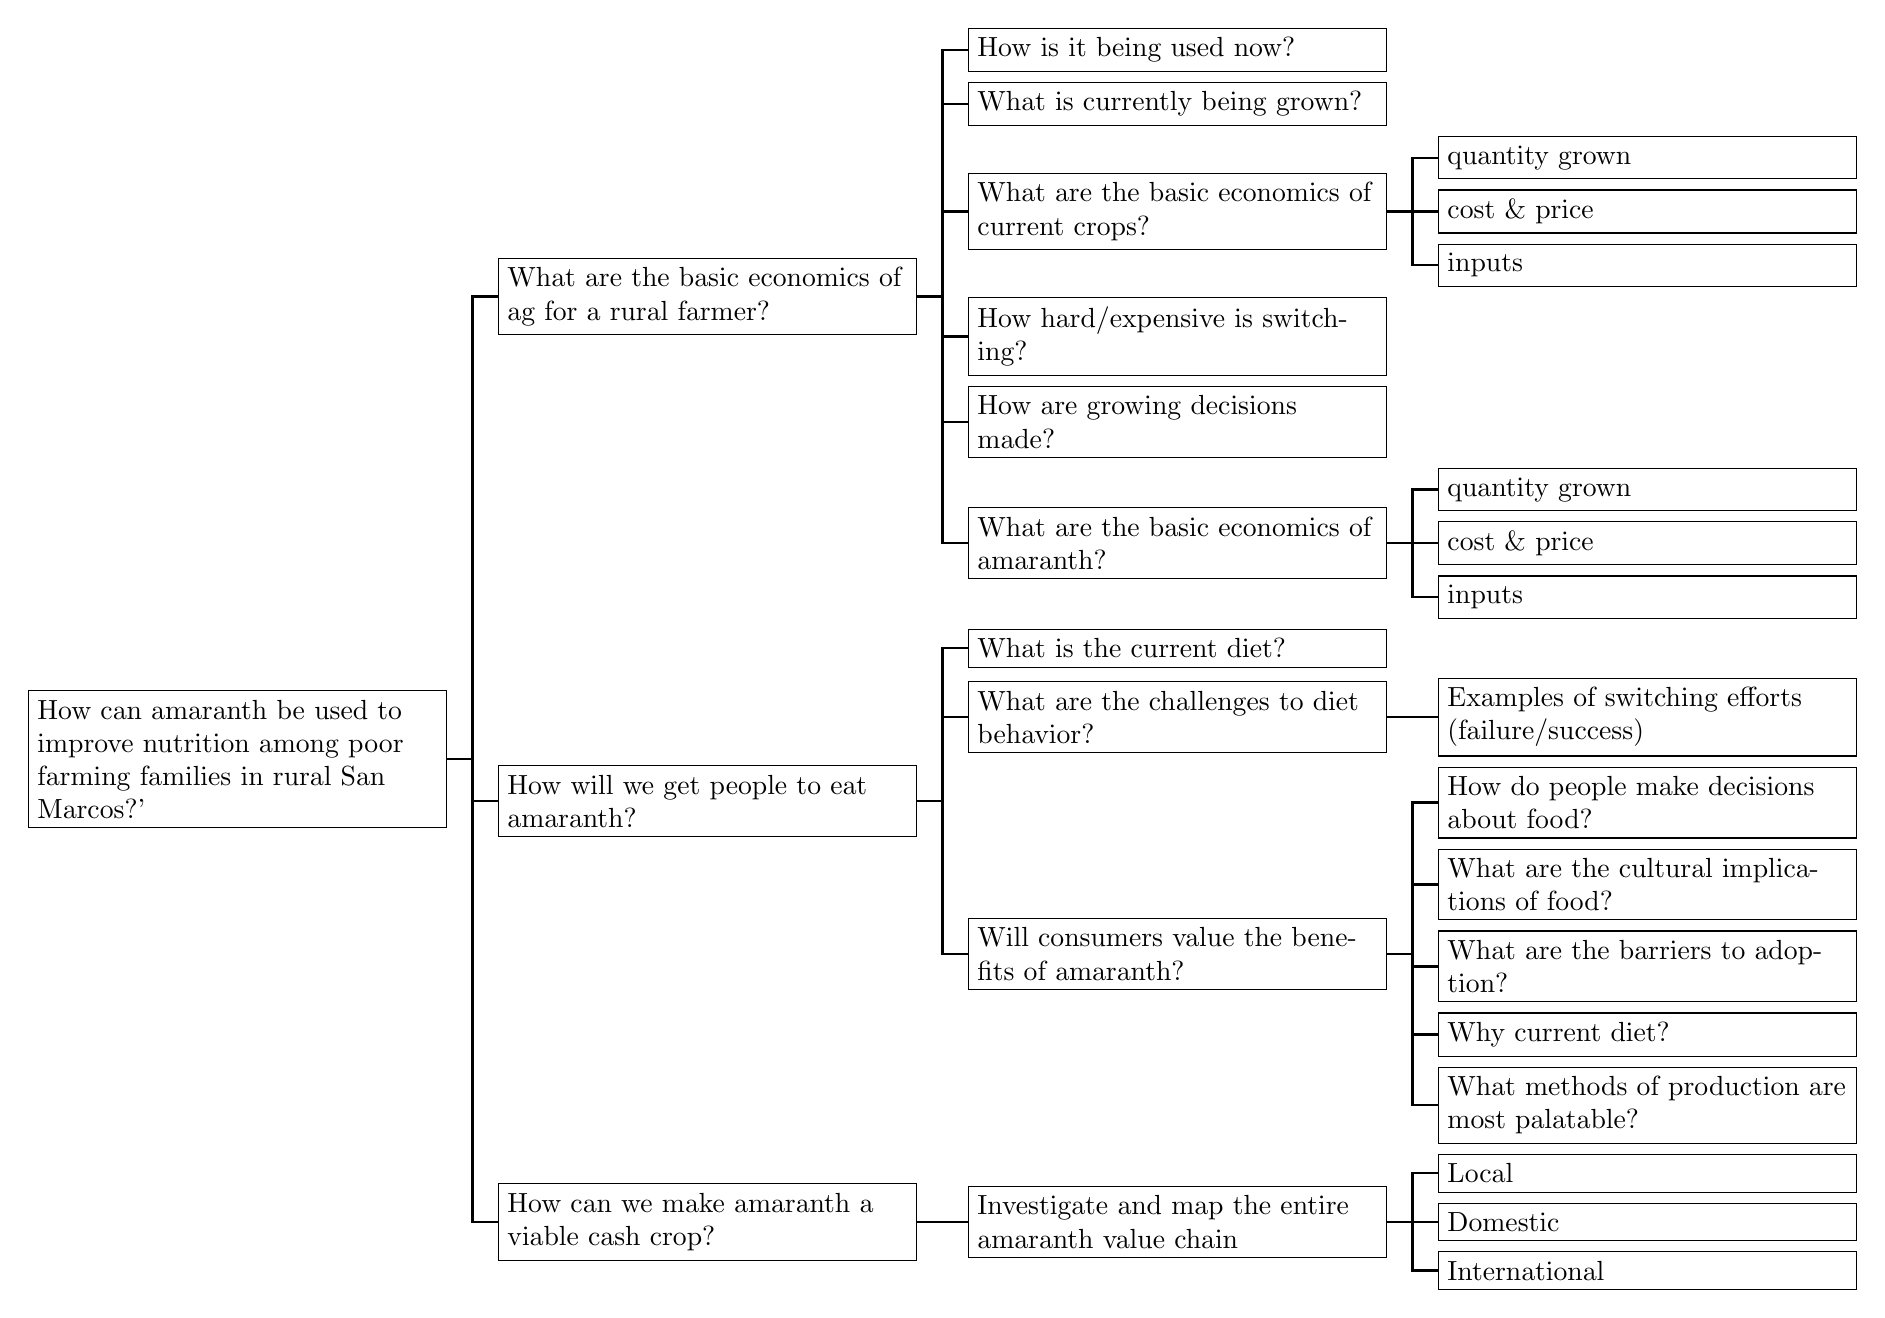
\begin{tikzpicture}[grow'=right,level distance=2.35in,sibling distance=.05in]
\tikzset{edge from parent/.style= 
            {thick, draw, edge from parent fork right},
         every tree node/.style=
            {draw,minimum width=1in,text width=2in,align=left}}
\Tree 
    [. {How can amaranth be used to improve nutrition among poor farming families in rural San Marcos?'} 
        [.{What are the basic economics of ag for a rural farmer?}
            [.{How is it being used now? } ]
            [.{What is currently being grown? } ]
            [.{What are the basic economics of current crops?} 
            	[.{quantity grown} ]            
            	[.{cost \& price} ]
           		[.{inputs} ]
            ]
            [.{How hard/expensive is switching? } ]
            [.{How are growing decisions made? } ]
            [.{What are the basic economics of amaranth? } 
            	[.{quantity grown} ]            
                [.{cost \& price} ]
                [.{inputs} ]
            ]
        ]
        [.{How will we get people to eat amaranth?}
            [.{What is the current diet? } ]
			[.{What are the challenges to diet behavior?} 
            	[.{Examples of switching efforts (failure/success)} ]            
            ]
 			[.{Will consumers value the benefits of amaranth?} 
            	[.{How do people make decisions about food?} ]            
            	[.{What are the cultural implications of food?} ]
           		[.{What are the barriers to adoption?} ]
           		[.{Why current diet?} ]
            [.{What methods of production are most palatable? } ]
            ]
        ] 
        [.{How can we make amaranth a viable cash crop?} 
        	[.{Investigate and map the entire amaranth value chain} 
                 [.{Local} ]            
                 [.{Domestic} ]
                 [.{International} ]
            ]
        ]
    ]
\end{tikzpicture}














\begin{comment}

\begin{thebibliography}{99}

\bibitem{nelson} Nelson, Robert C. \emph{Flight Stability and Automatic Control}. McGraw-Hill Companies, Inc., 1998. Print. 

\end{thebibliography}

\vspace{4 cm}



\clearpage
\section{Appendix A - {\tt{MATLAB}} Code}
\label{appx}


All {\tt{MATLAB}} functions used for computations related to this project are included in this appendix.  

\subsection{Script \tt{orbital\_final\_proj.m}}
\begin{lstlisting}
%%  AME 30381: Final Project
%   Jovian Lunar Cartography
tic
clear;clc;close all;
format compact;
set(0,'DefaultFigureWindowStyle','docked')

%% Define Planetary Objects
display('Defining Objects...')
% Define initial Earth object
% Earth is the default satellite object
Earth = satellite;

% Define initial Jupiter object
a = 778547.2;               % Mm
e = 0;                      % e_real = 0.048775
i = 0;                      % i_real = 1.305 deg
O = 100.492;                % deg
w = 275.066;                % deg
nu0 = 64.5;                 % Project document
epoch = 0;
mc = 1.98855e30;            % mass of Sun, kg
ms = 1.8986e27;             % mass of Jupiter, kg
rad = 69.911;               % Mm
Jupiter = satellite(a,e,i,O,w,nu0,epoch,mc,ms,rad);

\end{lstlisting}


\end{comment}
\end{document}